\section{Arithmetic Operations}

\begin{concept}{Processor Status Flags}\\
APSR (Application Program Status Register) contains important flags affected by arithmetic operations:
\begin{itemize}
  \item \textbf{N} (Negative): Set when result's MSB = 1, used for signed operations
  \item \textbf{Z} (Zero): Set when result = 0, used for both signed/unsigned
  \item \textbf{C} (Carry): Set when unsigned overflow occurs
  \item \textbf{V} (Overflow): Set when signed overflow occurs
\end{itemize}

Instructions ending with 'S' modify these flags:
\begin{itemize}
  \item ADDS, SUBS, MOVS, LSLS
\end{itemize}
\end{concept}

\begin{definition}{Basic Arithmetic Instructions}\\
Core arithmetic operations:
\begin{itemize}
  \item \textbf{ADD/ADDS}: Addition ($A + B$)
  \item \textbf{ADCS}: Addition with Carry ($A + B + c$)
  \item \textbf{ADR}: Address to Register ($PC + A$)
  \item \textbf{SUB/SUBS}: Subtraction ($A - B$)
  \item \textbf{SBCS}: Subtraction with carry/borrow ($A - B - !c$)
  \item \textbf{RSBS}: Reverse Subtract ($-1 \cdot A$)
  \item \textbf{MULS}: Multiplication ($A \cdot B$)
\end{itemize}
\end{definition}

\begin{definition}{Two's Complement}\\
For negative numbers:
\begin{itemize}
  \item Two's complement: $A = !A + 1$
  \item Used for representing signed numbers
  \item Enables using same hardware for addition and subtraction
\end{itemize}
\end{definition}

\begin{concept}{Carry and Overflow}\\
\textbf{Unsigned Operations:}
\begin{itemize}
  \item Addition: C = 1 indicates carry (result too large)
  \item Subtraction: C = 0 indicates borrow (result negative)
\end{itemize}

\textbf{Signed Operations:}
\begin{itemize}
  \item Addition: V = 1 if overflow with operands of same sign
  \item Subtraction: V = 1 if overflow with operands of opposite signs
\end{itemize}
\end{concept}

\begin{example2}{Multi-Word Addition}
Adding 96-bit values using ADCS:

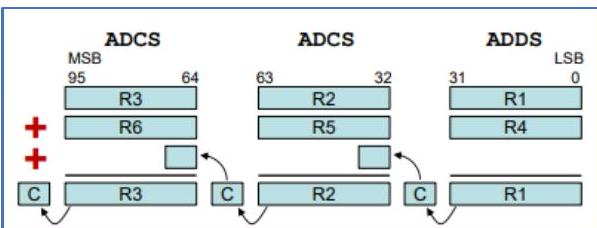
\includegraphics[width=\linewidth]{images/2024_12_29_79e6b22f503fb7b4f718g-04}

\begin{lstlisting}[language=armasm, style=basesmol]
    ADDS R1, R1, R4    ; Add least significant words
    ADCS R2, R2, R5    ; Add middle words with carry
    ADCS R3, R3, R6    ; Add most significant words with carry
\end{lstlisting}
\end{example2}

\begin{example2}{Multi-Word Subtraction}
Subtracting 96-bit values using SBCS:

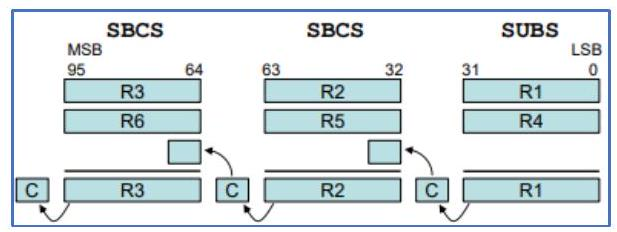
\includegraphics[width=\linewidth]{images/2024_12_29_79e6b22f503fb7b4f718g-04(1)}

\begin{lstlisting}[language=armasm, style=basesmol]
    SUBS R1, R1, R4    ; Subtract least significant words
    SBCS R2, R2, R5    ; Subtract middle words with borrow
    SBCS R3, R3, R6    ; Subtract most significant words with borrow
\end{lstlisting}
\end{example2}

\begin{example2}{Addition and Subtraction Examples}
Addition with carry (13d + 7d):
\begin{verbatim}
  1101  (13d)
  0111  (7d)
  ----
1 0100  (20d = 16d + 4d)
\end{verbatim}

Subtraction with borrow (6d - 14d):
\begin{verbatim}
  0110  (6d)
+ 0010  (TC of 14d)
  ----
  1000  (8d - 16d = -8d)
\end{verbatim}

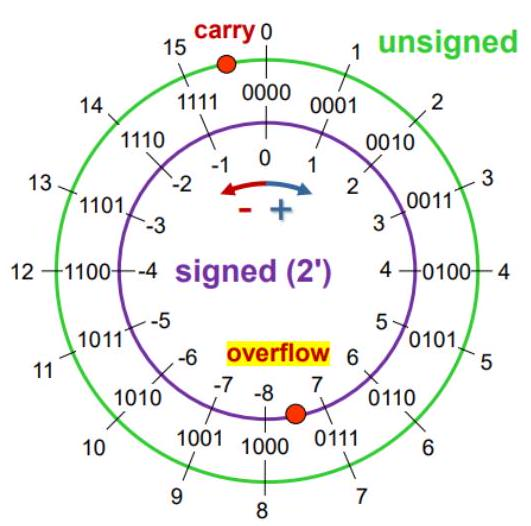
\includegraphics[width=\linewidth]{images/2024_12_29_79e6b22f503fb7b4f718g-04(2)}
\end{example2}

\begin{KR}{Arithmetic Operations}\\
Steps for arithmetic operations:
\begin{enumerate}
  \item Determine if operation is signed or unsigned
  \item Choose appropriate instruction (with or without 'S')
  \item Consider potential carry/overflow conditions
  \item For multi-word operations:
    \begin{itemize}
      \item Start with least significant words
      \item Use carry-aware instructions for higher words
      \item Track flags through operation
    \end{itemize}
  \item Check relevant flags after operation
\end{enumerate}
\end{KR}